\section{Durchführung}
\label{sec:Durchführung}

\subsection{Versuchsaufbau}
\label{sec:Versuchsaufbau}
%\begin{figure}
%	\centering
%	\caption{Schematische Darstellung des Versuchsaufbaus \cite{anleitung}.}
%	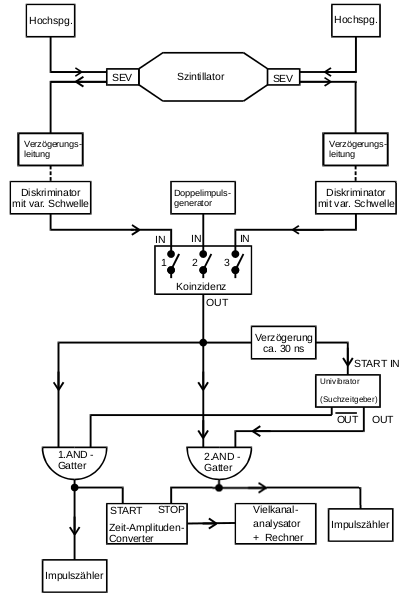
\includegraphics{Bilder/aufbau.png}
%	\label{fig:aufbau}
%\end{figure}
%
%\begin{figure}
%	\centering
%	\caption{Schematische Darstellung der Quelle zur Erzeugung radioaktiven Isotopen \cite{anleitung}.}
%	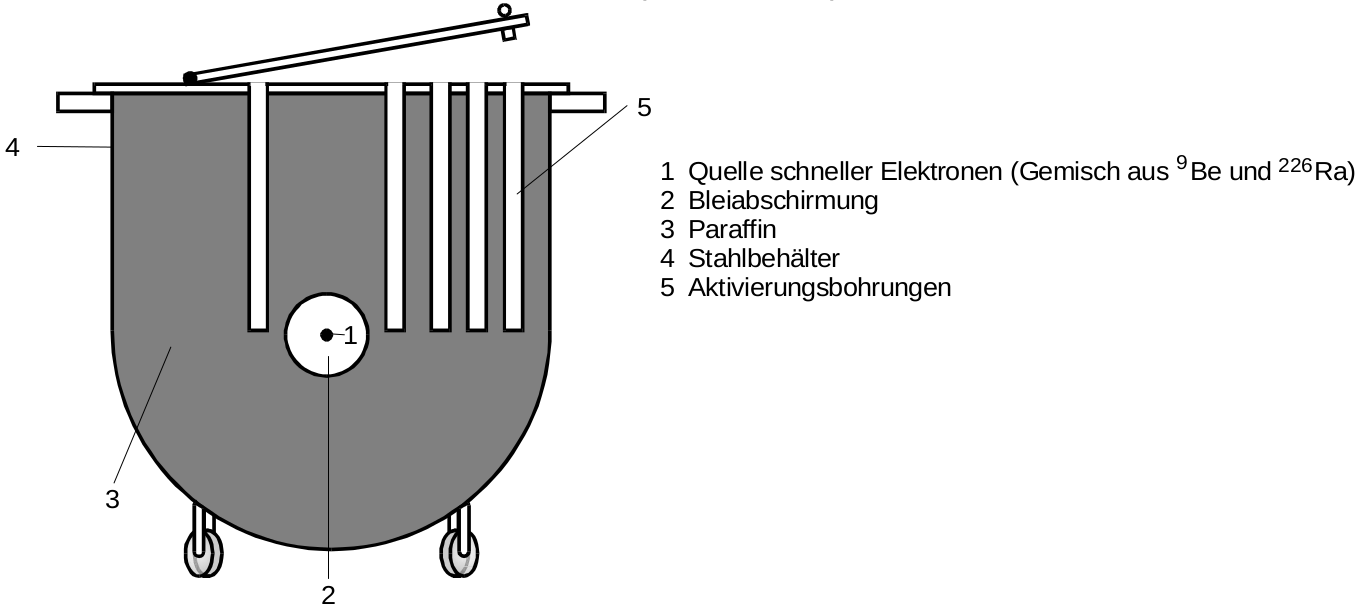
\includegraphics{content/toepfchen.png}
%	\label{fig:kochen}
%\end{figure}
%
Der Versuchsaufbau -- wie in Abbildung \ref{fig:aufbau} dargestellt -- besteht im Wesentlichen 
aus einem zerfallenden radioaktiven Isotop und einem Geiger-Müller-Zählrohr, welches die 
zerfallenden Kerne misst.
Das Geiger-Müller-Zählrohr ist entspricht einer mit Gas gefüllten Röhre. Trifft ein $\beta$-
oder $\gamma$- Teilchen auf ein Gasteilchen wird dieses ionisiert und kann aufgrund einer
anliegenden Spannung an der Röhre gemessen werden.
Dabei werden die gemessenen Zerfälle pro Messzeitintervall, welches am Zeitgeber einstellbar 
ist, an den Zählern 1 und 2 angezeigt. Nach jedem Messvorgang wird der Zähler umgeschaltet und 
der vorherige Wert auf dem aktuellen Zähler wird überschrieben. Der Versuchsaufbau ist mit
einer Blei-Abschirmung ausgestattet um die radioaktive Strahlung abzuschirmen.

Zur Erzeugung der radioaktiven Isotope wird das Objekt in Abbildung \ref{fig:kochen} verwendet.
Hierbei werden stabile Kerne mit niederenergetischen Neutronen beschossen. 
Da die Neutronen ihre Energie durch elastische Stöße an die Kerne übergeben und die maximale
Energie bei gleichen Massen der Stoßpartner erreicht wird, werden die Neutronen in einem 
Paraffinmantel gebremst, bis sie die optimale Energie besitzen.


\subsection{Versuchsbeschreibung}
\label{sec:Versuchsbeschreibung}

Vor Beginn der Messung werden die Kenngrößen der verwendeten Bauteile notiert.

Zur Bestimmung des effektiven Dämpfungswiderstandes $R_\text{eff}$ und der Abklingdauer $T_ex$ wird die Abnahme der Spannungsamplitude der Kondensatorspannung $U_\text{C}$ untersucht.
Es wird der kleinere der beiden fixen Widerstände des Schaltkreises, $R_\text{1}=(48.1 \pm 0.1)\,\si{\ohm}$, verwendet.
Dazu wird am Funktionengenerator ein Nadelimpuls eingestellt.
Die Kondensatorspannung wird hierbei auf den ersten Kanal des Oszilloskops gegeben.
Auf dem Bildschirm des Oszilloskops ist nun die Abnahme der Spannungsamplitude der Kondensators zu sehen.
Der Nadelimpuls soll nun so eingestellt werden, dass die Spannungsamplitude am Kondensator sich zwischen zwei Impulsen mindestens um den Faktor 3 bis 8 ändert.
Dazu werden die Frequenz und Amplitude des Nadelimpulses ebenso wie das Triggerlevel am Oszilloskop variiert, bis sich der gewünschte Spannungsverlauf auf dem Bildschirm des Oszilloskops zeigt.
Mit der Cursorfunktion werden nun die positiven Spannungsamplituden mit den zugehörigen Zeitdifferenzen zum auslösenden Nadelimpuls bestimmt und der Spannungsverlauf über die USB-Ausgabe des Oszilloskops gespeichert.

Für die zweite Messung zur Bestimmung des Widerstands $R_\text{ap}$ im aperiodischen Grenzfall wird der regelbare Widerstand $R_\text{3}$ verwendet.
Dieser wird zunächst auf seinen maximalen wert gestellt. Am Oszilloskop zeigt sich nun lediglich die erwartete stetig abfallende Spannung am Kondensator.
Der Widerstand $R_\text{3}$ wird nun so weit heruntergeregelt, dass am Spannungsverlauf Überschwinger sichtbar werden.
Der Widerstand $R_\text{3}$ wird nun langsam so weit wieder hoch geregelt, dass die Überschwinger soeben verwschwinden. Der Wert des Widerstandes $R_\text{3}$ entspricht nun dem Widerstand für den aperiodischen Grenzfall des Schaltkreises und wird notiert.

Zur Bestimmung der Frequenzabhängigkeit der Kondensatorspannung und der Phase zwischen Kondensator- und Erregerspannung wird am Funktionengenerator eine Sinusspannung eingestellt und die Generatorspannung $U(t)$ über den zweiten Kanal des Oszilloskops abgegriffen.
Am Oszilloskop werden beide Spannunsgverläufe übereinander gelegt.
Zunächst wird nun die Frequenz einmal über den Bereich $1 \,\si{\kilo\Hz}$ bis etwa $100 \,\si{\kilo\Hz}$ und dabei die Spannungsverläufe am Oszilloskop beobachtet, sodass etwa der Bereich der Resonatorfrequenz bestimmt werden kann.
Für Frequenzen nahe der Resonatorfrequenz wird im Weiteren in höherer Auflösung gemessen.
Es werden nun etwa 20 Datensätze aus Generatorspannung $U(t)$, Kondensatorspannung $U_\text{C}$, dem Abstand $a$ zwischen den Nulldurchgängen der beiden Spannungen und der jeweiligen Frequenz $f$ der Sinusspannung aufgenommen.
Die Spannungsmaxima beider Spannungen werden jeweils über die Measure-Funktion des Oszilloskops bestimmt.
Der Abstand zwischen den Nulldurchgängen der beiden Spannungsverläufe wird mit der Cursorfunktion bestimmt.
Die Periodenlänge $b$, welche zusätzlich zur Berechnung der Phasendifferenz $\phi$ benötigt wird, muss nicht gemessen werden, da sie über den Kehrwert der verwendeten Frequenz berechnet werden kann.
